\documentclass[12pt,letterpaper,titlepage]{report}
\usepackage{fontspec}
\defaultfontfeatures{Mapping=tex-text}
\usepackage{xunicode}
\usepackage{xltxtra}
\usepackage{enumitem}
\setmainfont{Times New Roman}
\usepackage{amsmath}
\usepackage{amsfonts}
\usepackage{amssymb}
\usepackage{multicol}
\usepackage{paracol}
\usepackage{graphicx}
\graphicspath{{img/}}
\usepackage{karnaugh-map}
\usepackage[margin=0.65in]{geometry}
\author{Jacob Abel}
\title{%
	Homework 5
	\\\large ECE2504 CRN:82729
}

\begin{document}
\maketitle
\begin{raggedright}
\raggedcolumns
\begin{multicols*}{2}
\paragraph{Question 1:}
(8 pts) For the Boolean functions E and F shown in the truth table below 

\begin{center}
\begin{tabular}{ c c c | c c | c | c }\hline
X & Y & Z & E & F & E+F &$E\bullet F$ \\\hline
0 & 0 & 0 & 1 & 0 & 1   & 0          \\\hline
0 & 0 & 1 & 0 & 1 & 1   & 0          \\\hline
0 & 1 & 0 & 0 & 0 & 0   & 0          \\\hline
0 & 1 & 1 & 1 & 1 & 1   & 1          \\\hline
1 & 0 & 0 & 1 & 0 & 1   & 0          \\\hline
1 & 0 & 1 & 1 & 1 & 1   & 1          \\\hline
1 & 1 & 0 & 0 & 1 & 1   & 0          \\\hline
1 & 1 & 1 & 0 & 0 & 0   & 0          \\\hline
\end{tabular}
\end{center}
\begin{enumerate} [label=\alph*)]
\item Express E in sum of minterms form
\begin{align*}
E&= X'Y'Z'+X'YZ\\&+XY'Z'+XY'Z
\end{align*}
\item Express F in sum of minterms form
\begin{align*}
F&= X'Y'Z+X'YZ\\&+XY'Z+XYZ'
\end{align*}
\item Express E in product of maxterms form
\begin{align*}
E= &(X+Y+Z')(X+Y'+Z)\\&(X'+Y'+Z)(X'+Y'+Z')
\end{align*}

\item Express F in product of maxterms form
\begin{align*}
F= &(X+Y+Z)(X+Y'+Z)\\&(X'+Y+Z)(X'+Y'+Z')
\end{align*}

\item Express $(E + F)$ in sum of minterms form 
\begin{align*}
(E+F)&= X'Y'Z'+X'Y'Z+X'YZ\\&+XY'Z'+XY'Z+XYZ'
\end{align*}
\item Express ($E \bullet F$) in product of maxterms form
\begin{align*}
(E\bullet F)= &(X+Y+Z)(X+Y+Z')
\\&(X+Y'+Z)(X'+Y+Z)
\\&(X'+Y'+Z)(X'+Y'+Z')
\end{align*}
\item Simplify E
  \begin{karnaugh-map}[4][2][1][$YZ$][$X$]
    \minterms{0, 3, 4, 5}
    \maxterms{1,2,6,7}
    \implicant{0}{4}
    \implicant{4}{5}
    \implicant{3}{3}
  \end{karnaugh-map}
  \begin{align*}
  E= Y'Z'+XY'+X'YZ
  \end{align*}
\item Simplify F
  \begin{karnaugh-map}[4][2][1][$YZ$][$X$]
    \minterms{0, 3, 4, 5}
    \maxterms{1,2,6,7}
    \implicant{1}{1}
    \implicant{2}{6}
    \implicant{7}{6}
  \end{karnaugh-map}
  \begin{align*}
  F= (X'+Y')(Y'+Z)(X+Y+Z')
  \end{align*}

\end{enumerate}
\end{multicols*}
\pagebreak

\paragraph{Question 2:}
(3 pts) Assume the gates in the circuit below have the following propagation delays. What is the propagation delay of the longest path through the circuit? Recall that $x \oplus y = x’y + xy’$
\begin{description}[noitemsep]
\item[Inverter] $t_{pd} = 0.05 ns$
\item[NAND gate] $t_{pd} = 0.07 ns$
\item[NOR gate] $t_{pd} = 0.07 ns$
\item[AND gate] $t_{pd} = 0.10 ns$
\item[OR gate] $t_{pd} = 0.10 ns$
\end{description}
\begin{center}
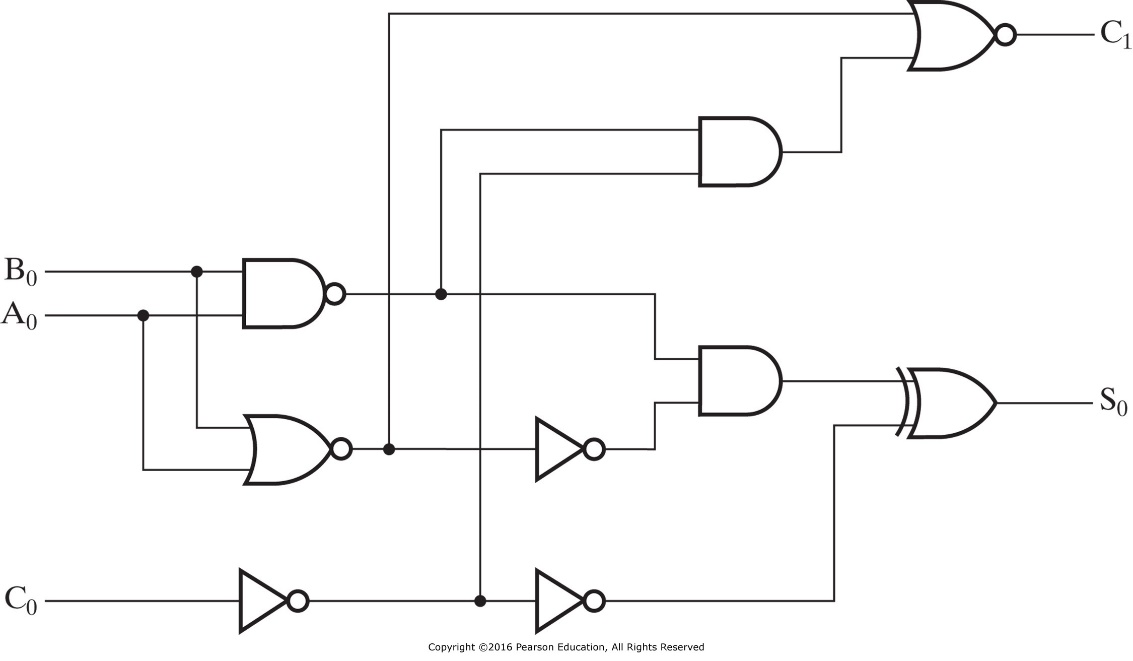
\includegraphics[width=0.8\columnwidth]{hw5p2}
\end{center}
The longest path is 

NOR -> NOT -> AND -> XOR. 

This path can be rendered into 

NOR -> NOT -> AND -> NOT -> AND -> OR 

by converting the xor gate into primitive gates.

\begin{align*}
t_{pd\; max} =& 0.07ns + 0.05ns + 0.10ns 
		   \\+& 0.05ns + 0.10ns + 0.10ns
		   \\
t_{pd\; max} =& 0.47ns
\end{align*}
\pagebreak

\paragraph{Question 3:}
Assume an electronic game uses an array of seven LEDs to display the results of a random roll of a die.  The value of each roll is represented by a 3‐bit binary number $X = X_2 X_1 X_0$.  Design a logic circuit to illuminate the appropriate LEDs to display each of the possible six die values, as shown below. The circuit outputs are a, b, c, d, e, f, and g. Assume the LEDs are active‐high. 

\includegraphics[width=\columnwidth]{hw5p3}

\begin{enumerate} [label=\alph*)]
\item (3.5 pts) Derive the truth table for a‐g. Assume that invalid input combinations (000 and 111) should result in all the LEDs remaining dark.

\begin{center}
\begin{tabular}{|c c c| c c c c c c c |}\hline
$X_2$ & $X_1$ & $X_0$ & a & b & c & d & e & f & g \\\hline
            0 & 0 & 0 & 0 & 0 & 0 & 0 & 0 & 0 & 0 \\\hline
            0 & 0 & 1 & 0 & 0 & 0 & 1 & 0 & 0 & 0 \\\hline
            0 & 1 & 0 & 1 & 0 & 0 & 0 & 0 & 0 & 1 \\\hline
            0 & 1 & 1 & 1 & 0 & 0 & 1 & 0 & 0 & 1 \\\hline
            1 & 0 & 0 & 1 & 1 & 0 & 0 & 0 & 1 & 1 \\\hline
            1 & 0 & 1 & 1 & 1 & 0 & 1 & 0 & 1 & 1 \\\hline
            1 & 1 & 0 & 1 & 1 & 1 & 0 & 1 & 1 & 1 \\\hline
            1 & 1 & 1 & 0 & 0 & 0 & 0 & 0 & 0 & 0 \\\hline
\end{tabular}
\end{center}

\item (3.5 pts) Determine simplified Boolean equations for a‐g.
\begin{paracol}{2}
\begin{karnaugh-map}[4][2][1][$X_1X_0$][$X_2$]
  \minterms{2,3,4,5,6}
  \autoterms[0]
  \implicant{4}{5}
  \implicant{3}{2}
  \implicant{2}{6}
\end{karnaugh-map}
\begin{align*}
a=X_2X_1'+X_2'X_1+X_1X_0'
\end{align*}
\switchcolumn
\begin{karnaugh-map}[4][2][1][$X_1X_0$][$X_2$]
  \minterms{4,5,6}
  \autoterms[0]
  \implicant{4}{5}
  \implicantedge{4}{4}{6}{6}
\end{karnaugh-map}
\begin{align*}
b=X_2X_1'+X_2X_0'
\end{align*}
\switchcolumn
\begin{karnaugh-map}[4][2][1][$X_1X_0$][$X_2$]
  \minterms{6}
  \autoterms[0]
  \implicant{6}{6}
\end{karnaugh-map}
\begin{align*}
c=X_2X_1X_0'
\end{align*}
\switchcolumn
\begin{karnaugh-map}[4][2][1][$X_1X_0$][$X_2$]
  \minterms{1,3,5}
  \autoterms[0]
  \implicant{1}{3}
  \implicant{1}{5}
\end{karnaugh-map}
\begin{align*}
d=X_1'X_0+X_2'X_0
\end{align*}
\switchcolumn
\begin{karnaugh-map}[4][2][1][$X_1X_0$][$X_2$]
  \minterms{6}
  \autoterms[0]
  \implicant{6}{6}
\end{karnaugh-map}
\begin{align*}
e=X_2X_1X_0'
\end{align*}
\switchcolumn
\begin{karnaugh-map}[4][2][1][$X_1X_0$][$X_2$]
  \minterms{4,5,6}
  \autoterms[0]
  \implicant{4}{5}
  \implicantedge{4}{4}{6}{6}
\end{karnaugh-map}
\begin{align*}
f=X_2X_1'+X_2X_0'
\end{align*}
\switchcolumn

\begin{karnaugh-map}[4][2][1][$X_1X_0$][$X_2$]
  \minterms{2,3,4,5,6}
  \autoterms[0]
  \implicant{4}{5}
  \implicant{3}{2}
  \implicant{2}{6}
\end{karnaugh-map}
\begin{align*}
g=X_2X_1'+X_2'X_1+X_1X_0'
\end{align*}

\end{paracol}
\item (2 pts) Implement a‐d using AND gates, OR gates, and inverters. (Assume a maximum of 4 inputs for each gate.)

\includegraphics[scale=0.45]{hw5p3c}

\item (2 pts) Implement a‐d using only 2‐input NAND gates. 
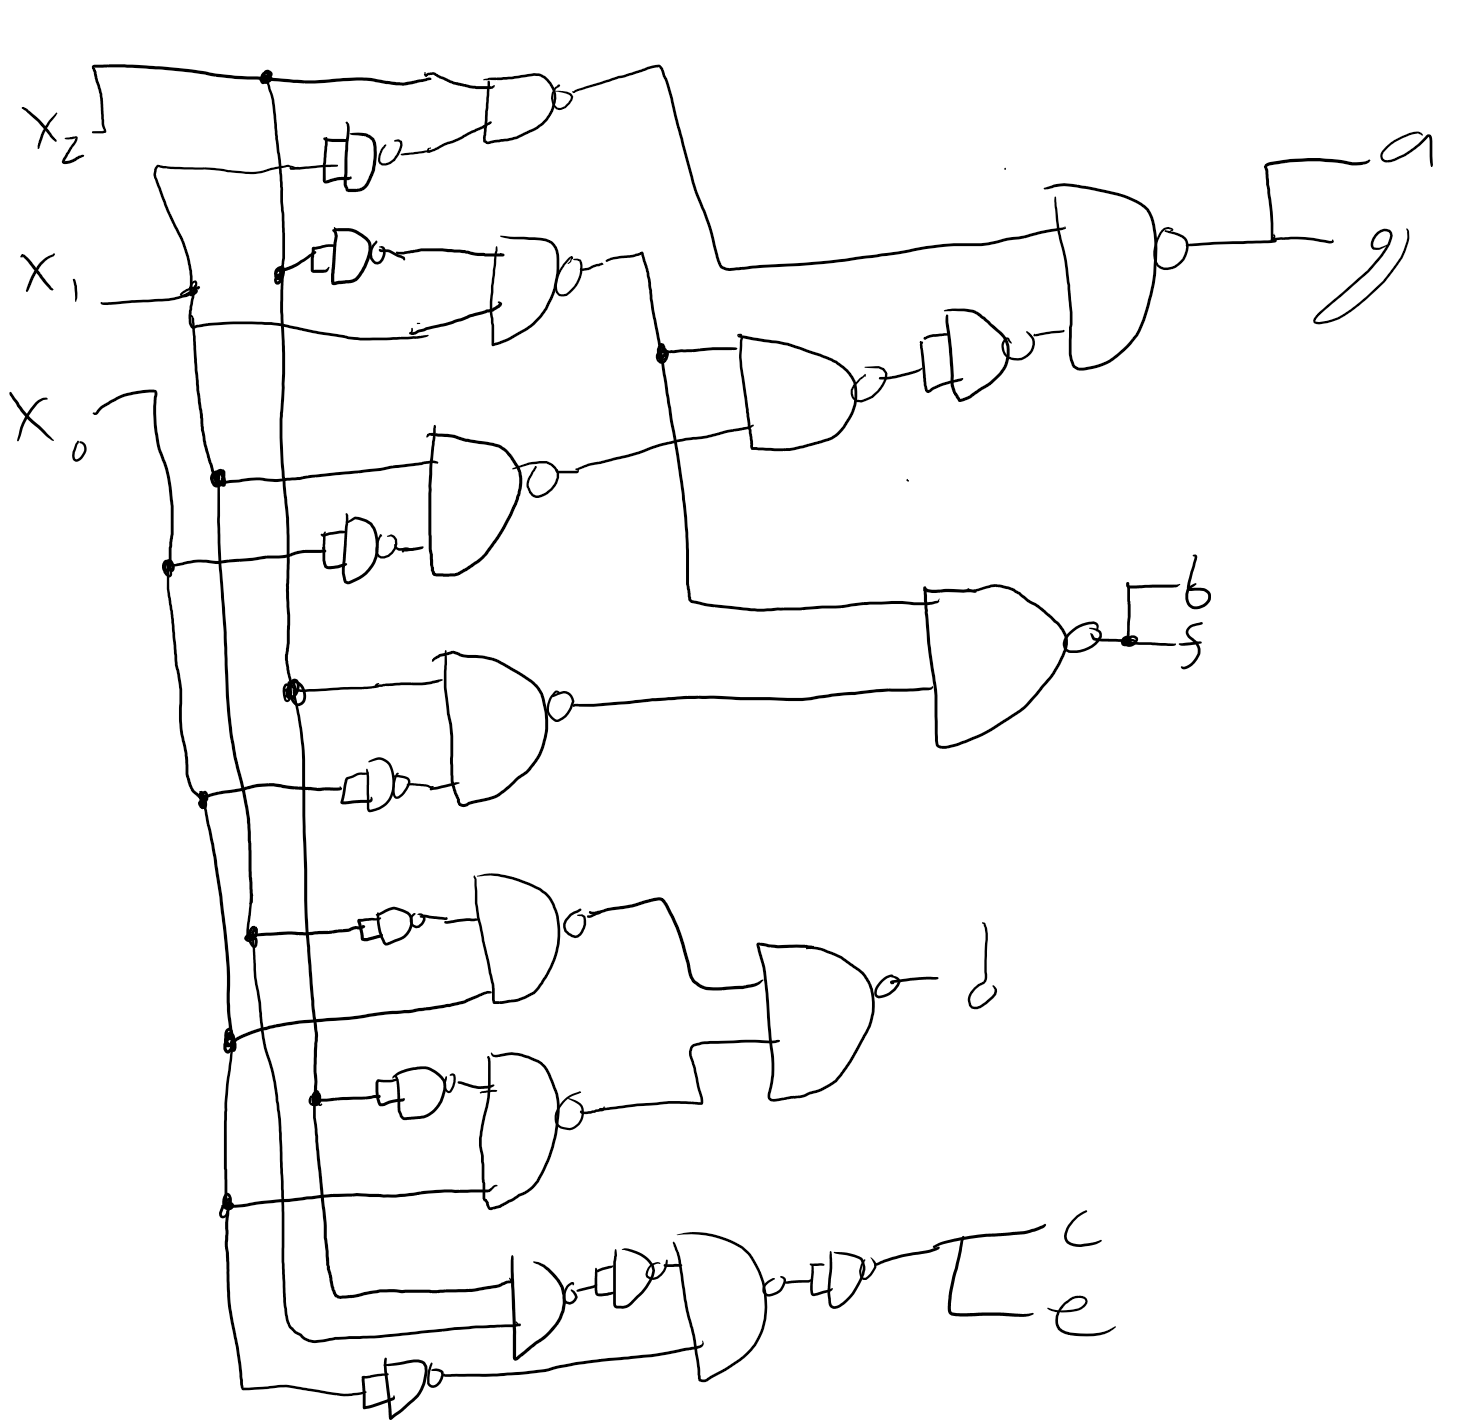
\includegraphics[scale=0.6]{hw5p3d}

\end{enumerate}
\pagebreak

\paragraph{Question 4:}
Modify the truth table from Problem 3 by assuming that an output is not specified for invalid input combinations. 
\begin{enumerate} [label=\alph*)]
\item (2 pts) Derive the modified truth table for a‐g.
\begin{center}
\begin{tabular}{|c c c| c c c c c c c |}\hline
$X_2$ & $X_1$ & $X_0$ & a & b & c & d & e & f & g \\\hline
            0 & 0 & 0 & x & x & x & x & x & x & x \\\hline
            0 & 0 & 1 & 0 & 0 & 0 & 1 & 0 & 0 & 0 \\\hline
            0 & 1 & 0 & 1 & 0 & 0 & 0 & 0 & 0 & 1 \\\hline
            0 & 1 & 1 & 1 & 0 & 0 & 1 & 0 & 0 & 1 \\\hline
            1 & 0 & 0 & 1 & 1 & 0 & 0 & 0 & 1 & 1 \\\hline
            1 & 0 & 1 & 1 & 1 & 0 & 1 & 0 & 1 & 1 \\\hline
            1 & 1 & 0 & 1 & 1 & 1 & 0 & 1 & 1 & 1 \\\hline
            1 & 1 & 1 & x & x & x & x & x & x & x \\\hline
\end{tabular}
\end{center}
 
\item (2 pts) Determine simplified Boolean equations for a‐d using the new truth table. 
\begin{paracol}{2}
\begin{karnaugh-map}[4][2][1][$X_1X_0$][$X_2$]
  \minterms{2,3,4,5,6}
  \indeterminants{0,7}
  \autoterms[0]
  \implicant{3}{6}
  \implicant{4}{6}
\end{karnaugh-map}
\begin{align*}
a=X_2+X_1
\end{align*}
\switchcolumn
\begin{karnaugh-map}[4][2][1][$X_1X_0$][$X_2$]
  \minterms{4,5,6}
  \indeterminants{0,7}
  \autoterms[0]
  \implicant{0}{4}
  \implicant{4}{6}
\end{karnaugh-map}
\begin{align*}
b=X_2+X_1'X_0'
\end{align*}
\switchcolumn
\begin{karnaugh-map}[4][2][1][$X_1X_0$][$X_2$]
  \minterms{6}
  \indeterminants{0,7}
  \autoterms[0]
  \implicant{7}{6}
\end{karnaugh-map}
\begin{align*}
c=X_2X_1
\end{align*}
\switchcolumn
\begin{karnaugh-map}[4][2][1][$X_1X_0$][$X_2$]
  \minterms{1,3,5}
  \indeterminants{0,7}
  \autoterms[0]
  \implicant{1}{7}
\end{karnaugh-map}
\begin{align*}
d=X_0
\end{align*}
\switchcolumn
\begin{karnaugh-map}[4][2][1][$X_1X_0$][$X_2$]
  \minterms{6}
  \indeterminants{0,7}
  \autoterms[0]
  \implicant{7}{6}
\end{karnaugh-map}
\begin{align*}
e=X_2X_1
\end{align*}
\switchcolumn
\begin{karnaugh-map}[4][2][1][$X_1X_0$][$X_2$]
  \minterms{4,5,6}
  \indeterminants{0,7}
  \autoterms[0]
  \implicant{0}{4}
  \implicant{4}{6}
\end{karnaugh-map}
\begin{align*}
f=X_2+X_1'X_0'
\end{align*}
\switchcolumn

\begin{karnaugh-map}[4][2][1][$X_1X_0$][$X_2$]
  \minterms{2,3,4,5,6}
  \indeterminants{0,7}
  \autoterms[0]
  \implicant{3}{6}
  \implicant{4}{6}
\end{karnaugh-map}
\begin{align*}
g=X_2+X_1
\end{align*}

\end{paracol}
  
\item (2 pts) Implement a‐d using AND gates, OR gates, and inverters using the new expressions. (Assume a maximum of 4 inputs for each gate.) 

\includegraphics[scale=0.8]{hw5p4c}

\item (2 pts) Implement a‐d using only 2‐input NAND gates.
\includegraphics[scale=0.6]{hw5p4d}

 
\end{enumerate}
\pagebreak

\paragraph{Question 5:}
(8 pts) Minimize the following five variable function. 
\begin{align*}
F(A,B,C,D,E)=\Sigma(&0,8,9,10,12,14,15,16,
		   		\\& 20,24,27,29,31)\\
d(A,B,C,D,E)=\Sigma(&4,7,11,13,19,25,28, 30)
\end{align*}

Hint: Consider a 4‐variable K‐map.  It consists of 16 cells, arranged so that adjacent cells differ by only one variable. Suppose a second 4‐variable K‐map is stacked on top of the first. Differentiate between the top K‐map and the bottom K‐map using a fifth bit, e.g. 0 for the bottom, 1 for the top. This will be the most significant bit of your 5‐variable K‐map. 

\begin{karnaugh-map}[4][4][2][$CD$][$AB$][$E$]
  \minterms{0,8,9,10,12,14,15,16,20,24,27,29,31}
  \indeterminants{4,7,11,13,19,25,28,30}
  \autoterms[0]
  \implicant{0}{8}[0,1]
  \implicant{12}{10}[0]
  \implicant{13}{11}[0,1]
\end{karnaugh-map}
\begin{align*}
F=& C'D'+AD+AE'
\end{align*}

\bigskip
\noindent
GRADING SCALE
\medskip

Total: 38 pts
\bigskip

\def\arraystretch{1.5} 
\begin{tabular}{ | l | c | c | c | c | c | c | c | c | } \hline
Pts          & 0  & 4  & 9  & 14 & 19 & 23 & 28 & 33     \\\hline
Letter Grade & D- & D  & C- & C  & B- & B  & A- & A      \\\hline
\end{tabular}
\end{raggedright}
\end{document}